\PassOptionsToPackage{unicode=true}{hyperref} % options for packages loaded elsewhere
\PassOptionsToPackage{hyphens}{url}
%
\documentclass[]{article}
\usepackage{lmodern}
\usepackage{amssymb,amsmath}
\usepackage{ifxetex,ifluatex}
\usepackage{fixltx2e} % provides \textsubscript
\ifnum 0\ifxetex 1\fi\ifluatex 1\fi=0 % if pdftex
  \usepackage[T1]{fontenc}
  \usepackage[utf8]{inputenc}
  \usepackage{textcomp} % provides euro and other symbols
\else % if luatex or xelatex
  \usepackage{unicode-math}
  \defaultfontfeatures{Ligatures=TeX,Scale=MatchLowercase}
\fi
% use upquote if available, for straight quotes in verbatim environments
\IfFileExists{upquote.sty}{\usepackage{upquote}}{}
% use microtype if available
\IfFileExists{microtype.sty}{%
\usepackage[]{microtype}
\UseMicrotypeSet[protrusion]{basicmath} % disable protrusion for tt fonts
}{}
\IfFileExists{parskip.sty}{%
\usepackage{parskip}
}{% else
\setlength{\parindent}{0pt}
\setlength{\parskip}{6pt plus 2pt minus 1pt}
}
\usepackage{hyperref}
\hypersetup{
            pdftitle={Effect of Mandatory Jail Sentences on Vehicle Fatality Rates},
            pdfborder={0 0 0},
            breaklinks=true}
\urlstyle{same}  % don't use monospace font for urls
\usepackage[margin=1in]{geometry}
\usepackage{longtable,booktabs}
% Fix footnotes in tables (requires footnote package)
\IfFileExists{footnote.sty}{\usepackage{footnote}\makesavenoteenv{longtable}}{}
\usepackage{graphicx,grffile}
\makeatletter
\def\maxwidth{\ifdim\Gin@nat@width>\linewidth\linewidth\else\Gin@nat@width\fi}
\def\maxheight{\ifdim\Gin@nat@height>\textheight\textheight\else\Gin@nat@height\fi}
\makeatother
% Scale images if necessary, so that they will not overflow the page
% margins by default, and it is still possible to overwrite the defaults
% using explicit options in \includegraphics[width, height, ...]{}
\setkeys{Gin}{width=\maxwidth,height=\maxheight,keepaspectratio}
\setlength{\emergencystretch}{3em}  % prevent overfull lines
\providecommand{\tightlist}{%
  \setlength{\itemsep}{0pt}\setlength{\parskip}{0pt}}
\setcounter{secnumdepth}{5}
% Redefines (sub)paragraphs to behave more like sections
\ifx\paragraph\undefined\else
\let\oldparagraph\paragraph
\renewcommand{\paragraph}[1]{\oldparagraph{#1}\mbox{}}
\fi
\ifx\subparagraph\undefined\else
\let\oldsubparagraph\subparagraph
\renewcommand{\subparagraph}[1]{\oldsubparagraph{#1}\mbox{}}
\fi

% set default figure placement to htbp
\makeatletter
\def\fps@figure{htbp}
\makeatother

\usepackage{float}
\let\origfigure\figure
\let\endorigfigure\endfigure
\renewenvironment{figure}[1][2] {
    \expandafter\origfigure\expandafter[H]
} {
    \endorigfigure
}

\title{Effect of Mandatory Jail Sentences on Vehicle Fatality Rates}
\author{}
\date{\vspace{-2.5em}}

\begin{document}
\maketitle

Team ID: Team 6

NAME: Connor Rosenberg
NAME: Rongkui Han
NAME: Yuqing Yang
NAME: Nassim Ali-Chaouche

Github: \url{https://github.com/STA207/Presentation}

\hypertarget{introduction}{%
\section{Introduction}\label{introduction}}

\hypertarget{background}{%
\subsection{Background}\label{background}}

Traffic accidents cause thousands of deaths in the United States every year. Data pertinent to US traffic fatalities from 1982 to 1988 can be easily accessed in the AER ``Fatalities'' dataset. The data was obtained from sources such as the US Department of Transportation Fatal Accident Reporting System (FARS) and the US Bureau of Labor Statistics. The dataset includes panel data for 48 states (Alaska and Hawaii not included), containing demographic variables such as population, income per capita, religious belief, and unemployment rate. In addition, features that are commonly associated with traffic accidents and its regulation, such as average miles per driver, percentage of young drivers, tax collected per case of beer, presence of a preliminary breath test law, and whether the state implemented mandatory jail sentences or community service for an initial drunk driving conviction, were also presented in the dataset. Finally, the number of vehicle fatalities and its numerous subsets, such as night-time or single-vehicle fatalities, were introduced. The observations were recorded for each state annually. In total, there are 336 observations recorded for 34 distinct variables.

Due to the observational nature of the data, obtaining causal effects may pose a challenge. In observational studies, treatment selection is influenced by subject characteristics. In the context of our study, ``treatment assignment'' refers to whether a state has a mandatory jail sentence. It is not difficult to imagine that demographic characteristics of a state can influence both its traffic legislations as well as its traffic fatality rate, causing confounding effects. As a result, systematic differences in baseline characteristics between states with and without mandatory jail sentences must be taken into account when estimating its effect on outcomes. The \textbf{propensity score} is the probability of treatment assignment conditional on observed baseline characteristics. The propensity score allows one to analyze an observational study so that it mimics some of the particular characteristics of a randomized controlled trial. In particular, conditional on the propensity score, the distribution of observed baseline covariates will be similar between treated and untreated subjects, allowing the estimation of the average treatment effect (Austin, 2011). In this report, we will attempt to discover the potential causal relationship between mandatory jail sentences and State traffic fatality rate using propensity score matching, followed by mixed-effect ANOVA modeling.

\hypertarget{questions-of-interest}{%
\subsection{Questions of Interest}\label{questions-of-interest}}

\begin{itemize}
\tightlist
\item
  Are there demographic features that correlate with a state's mandatory jail sentence law?\\
\item
  Is a state's mandatory jail sentence law associated with its annual traffic fatality rate, after adjusting for potential covariating demographic variables?\\
\item
  Can we draw a causal conclusion regarding the relationship between a state's mandatory jail sentence law and its annual traffic fatality rate?
\end{itemize}

\hypertarget{analysis-plan}{%
\section{Analysis Plan}\label{analysis-plan}}

\hypertarget{population-and-study-design}{%
\subsection{Population and Study Design}\label{population-and-study-design}}

The response variable used in this analysis is the yearly traffic fatality rate per 10,000 State residents. The ``Fatalities'' dataset is a panel dataset from 1982 to 1988. In a typical panel dataset, each subject has multiple entries, some of which correspond to pre-treatment records while others post-treatment. In this regard, the vehicle fatality dataset is atypical, because only six out of 48 states had pre- and post-treatment records (Figure \ref{fig:fatal}). In fact, most states did not change their policy. Due to this limitation, common panel data analysis techniques are not applicable. In response, we will follow a bench-marked pipeline for analyzing non-panel observational data under a propensity score matching framework (Smith, 1997).

\hypertarget{propensity-score-analysis}{%
\subsection{Propensity Score Analysis}\label{propensity-score-analysis}}

\hypertarget{propensity-score-estimation}{%
\subsubsection{Propensity Score Estimation}\label{propensity-score-estimation}}

We will estimate the propensity score through a logistic regression model. The dependent variable is binary, indicating treatment status. There is a lack of consensus in the literature as to which variables to include in the propensity score model (Austin, 2001). Brookhart et al. (2006) suggested that for practical purposes, it is safe to include all potential confounding covariables in propensity score estimation. In this study, 14 independent variables were included to account for demographic characteristics that could potentially influence whether a state mandates such a jail sentence. These variables include year, population, gross state product (GSP), spirits consumption, unemployment rate, per capita income, tax on a case of beer, percentage of baptists, percentage of Mormons, minimum drinking age, percent residing in dry counties, percentage of drivers younger than 24, average miles per driver, and preliminary breath test upon initial drunk driving conviction.

The output of this model is the propensity score, which equals to the probability that a State has a mandatory jail sentence given the set of covariates. The logistic regression model we used to estimate the propensity score is as follows:

\[
log(\frac{\pi_i}{1-\pi_i}) = \beta_0 + \beta_1x_{i1} + ... + \beta_kx_{ik}, 
\]
Where \(\pi_i = P(Z_i = 1 | \overrightarrow{X_i} = \overrightarrow{x_i})\), \(Z_i\) is the indicator variable for mandatory jail sentence upon initial drunk driving conviction. \(Z_i = 1\) when the state has mandatory jail sentence, and \(Z_i = 0\) other wise. \(\overrightarrow{X_i}\) is a vector of length 14, indicating the realized value of the 14 independent variables of the i-th subject in the logistic regression model. \(k = 1, ..., 15, i = 1,...,336\).

\hypertarget{matching}{%
\subsubsection{Matching}\label{matching}}

To match observations with mandatory jail sentences to observations without, we will use the nearest neighbor matching algorithm based upon propensity score.

After the propensity score matching, we would check whether our propensity score model has been adequately specified by comparing the distributions of the covariates between treatments.

\hypertarget{estimating-treatment-effect}{%
\subsubsection{Estimating Treatment Effect}\label{estimating-treatment-effect}}

There are two primary challenges in our analysis. First, fatality rates are likely correlated between states who share a \textbf{geographic boundary}. For example, the States of New York and New Jersey share many of the same commutors, which correlate their traffic fatality rates. Secondly, there is a likely correlation in a State's fatality rate \textbf{across time}. To mediate the effects of spatial correlations in our dataset, we introduced a ``region'' variable that categorizes states by their location. We included both the region and year variables as fixed effects in our model for estimating jail sentence treatment effect.

While these procedures are expected to control for some of the correlations, they are by no means comprehensive. We expect some of biases to remain in the results.

To estimate the effect of mandatory jail sentences on a State's traffic fatality rate, we will fit the following linear regression relating the binary treatment variable to Fatality Rate:

\[
Y_{ijkl} = \mu + \alpha_i + \beta_j  + \gamma_k + \epsilon_{ijkl}
\]
for \(i \in [Northeast, Midwest, South, West],\) \(j \in [1982, 1983, ..., 1988],\) \(k \in [0, 1],\) and \(l \in [1, ..., n_{ijk}]\).

Where\\
- \(Y_{ijkl}\) represents the yearly traffic fatality rate of a given state in a given year.\\
- \(\mu\) represents the overall sample mean of fatality rates.\\
- \(\alpha_i\) represents the fixed effect of geographical region \(i\).\\
- \(\beta_j\) represents the fixed effect of year. Note that year is treated as a categorical variable, not a numerical variable.\\
- \(\gamma_k\) represents the fixed effect of mandatory jail sentence law. \(k = 1\) when the state has mandatory jail sentence, and \(k = 0\) other wise.\\
- \(\epsilon_{ijkl}\) is the error.

The model is constrained such that \(\displaystyle\sum\limits_{i = 0, 1}\alpha_i = 0\), \(\displaystyle\sum\limits_{i = 0, 1}\beta_j = 0\), \(\displaystyle\sum\limits_{i = 0, 1}\gamma_k = 0\), and \(\epsilon_{ijklm} \overset{\text{iid}}\sim N(0, \sigma^2)\).

\hypertarget{horvitz-thompson-inverse-probability-weighting}{%
\subsubsection{Horvitz-Thompson Inverse-Probability Weighting}\label{horvitz-thompson-inverse-probability-weighting}}

To estimate the average treatment effect of jail sentences, we will also use the Horvitz-Thompson Weighting method, which balances the weighted distribution of covariates in the two groups. One of the advantages of Horvitz-Thompson weighting is that we could use all available data. Considering that the observation with propensity scores close to 0 or 1 will have unstable weights, leading to potentially spurious treatment effects with high variance, we will first truncate the propensity scores from 0.1 to 0.9.

Let \(Y_i\) denote the yearly traffic fatality rate of subject \(i\), \(Z_i\) denote the jail sentence status of subject \(i\), \(Z_i = 1\) when the state has mandatory jail sentence, and \(Z_i = 0\) other wise. \(\overrightarrow{X_i}\) is a vector of length 14, indicating the realized value of the 14 independent variables of the \(i\)-th subject in the logistic regression model. \(e(X) = Pr(Z = 1 | X)\) is the propensity score of subject \(i\).

Then the average treatment effect (ATE) \(\tau^{ATE}\) can be calculated by:

\[
\tau^{ATE} = \mathbb{E}[\frac{ZY}{e(X)} - \frac{(1-Z)Y}{1-e(X)}]
\]

Define Horvits-Thompson inverse-pronbability weight as:

\[
w_1(X_i) = \frac{1}{e(X_i)}, for Z_i = 1 \\
w_0(X_i) = \frac{1}{1-e(X_i)}, for Z_i = 0
\]
Then an unbiased non-parametric estimator of ATE is:

\[
\hat{\tau}^{ATE} = \frac{\displaystyle\sum\limits_iY_iZ_iw_1(X_i)}{\displaystyle\sum\limits_iZ_iw_1(X_i)} - \frac{\displaystyle\sum\limits_iY_i(1-Z_i)w_0(X_i)}{\displaystyle\sum\limits_i(1-Z_i)w_0(X_i)}
\]

The Horvitz-Thompson inverse-probability weighting will provide another propensity-score based measure for the average effect of mandatory jail sentences.

\hypertarget{model-diagnostics}{%
\subsection{Model Diagnostics}\label{model-diagnostics}}

We will use Q-Q plot, histogram and the Shapiro-Wilk test inspect the normality of residuals.to inspect the normality of residuals. A residuals-versus-fitted value scatter plot will be used to examine equality of residual variance. Influential observations will also be discussed.

\hypertarget{causal-inference-assumptions}{%
\subsection{Causal Inference Assumptions}\label{causal-inference-assumptions}}

A State legislature's decision to implement this policy is based upon much of the information contained within our dataset. This creates a dependence between the assigned treatment level and our other predictor variables. We control for this by conditioning on the covariates which affect the outcome and treatment selection through propensity score matching. (Sasidharan, 2013).

To make causal inferences with propensity score analysis, we make the following assumptions:

\textbf{Stable unit treatment value assumption (SUTVA)} (Rubin, 1990): This assumption states that the treatment applied to one entity does not affect the outcome of any other. In our case, it is challenging to make this assumption due to the aforementioned spacial and temporal correlations present in the dataset. For the purpose of this project, we will assume that including the ``region'' and ``year'' variables in the mixed effect model controls for the underlying bias.

\textbf{Positivity}: This assumption requires that there be a non-zero probability of receiving every level of treatment for the combination of values among entities in the population (Rubin, 1978). Since each state can pass legislation for and against mandatory jail sentences at any time, the probability of receiving both levels of the treatment is, in fact, positive.

\textbf{Unconfoundedness}: The treatment assignment mechanism is said to be unconfounded if the treatment status is conditionally independent of the potential outcomes, given a set of covariates (Rubin, 1990). This assumption is not satisfied by our original data since a clear dependence exists between a State's decision to implement mandatory jail sentences is based upon much of the data we plan to use in our analysis. However, propensity score matching will control for this since the propensity score is conditioned on all potential covariates (Rosenbaum, 1983).

\textbf{Observation of all Covariates}: This assumption, unique to propensity score, requires we observe all possible covariates in the assignment of a treatment (Rosenbaum, 1983). With such a complex decision such as implementing a required jail sentence, it is impossible to assume that our data is a complete case of all covariates. However, since we are limited with both the data and time at hand, we will make this assumption in order to continue the project.

\hypertarget{results}{%
\section{Results}\label{results}}

\hypertarget{descriptive-analysis}{%
\subsection{Descriptive Analysis}\label{descriptive-analysis}}

The distribution of traffic fatality rate is not even across state borders (Figure \ref{fig:map}). First, we found out there is an incomplete observation. The observation for California in 1988 did not include information on if the State mandated a jail sentence. We attempted to research the value but could not find a definitive answer. Therefore, we removed the observation. Of the 48 States included, 41 did not change their policy from 1982 to 1988. The fatality rates of the seven states who did change their policy is shown in Figure \ref{fig:fatal}(a). Both South Carolina and Nevada changed their policy in the mandatory jail sentence from no to yes in 1983, but their fatality rates changed in the opposite direction. Similarly, we can also observe this same situation in Oregon, Utah, and Connecticut.

\begin{figure}
\centering
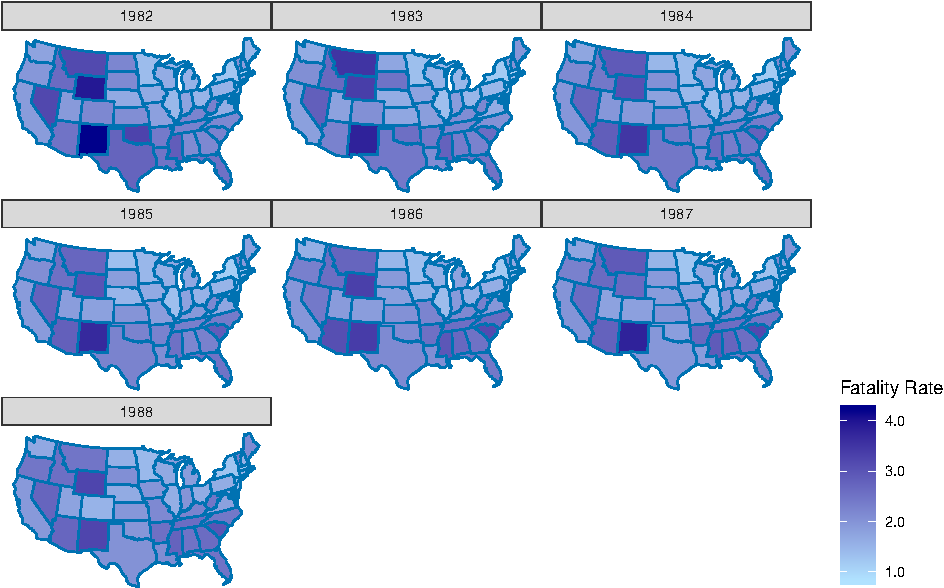
\includegraphics{team6_final_project_3_files/figure-latex/map-1.pdf}
\caption{\label{fig:map}State traffic fatality rate per 10,000 population in years 1982-1988}
\end{figure}

Then, we explore the distribution of fatalities rate across all observations. Figure \ref{fig:fatal}(b) shows that overall, states that had a mandatory jail sentence had a higher fatality rate than states that did not. Figure \ref{fig:fatal}(c) shows that distributions of fatalities rate for different years are roughly the same.

\begin{figure}
\centering
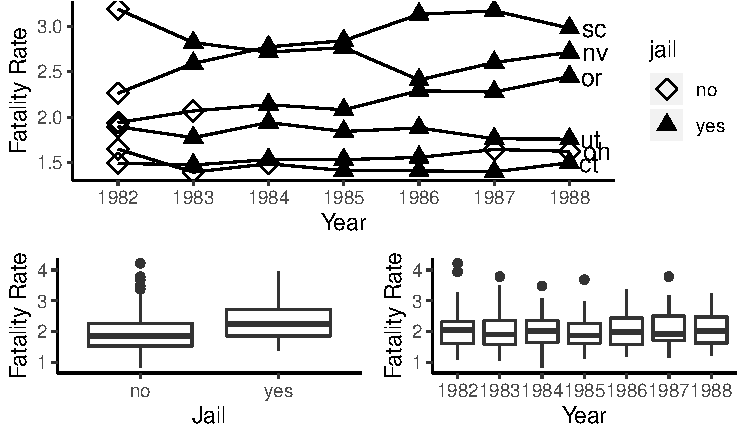
\includegraphics{team6_final_project_3_files/figure-latex/fatal-1.pdf}
\caption{\label{fig:fatal}(a) Fatality rate for states that changed their policy in the mandatory jail sentence from 1982 to 1988 (b) Boxplot of the fatality rate for different policies in the mandatory jail sentence (c) Boxplot of the fatality rate for different years}
\end{figure}

\hypertarget{propensity-score-analysis-1}{%
\subsection{Propensity Score Analysis}\label{propensity-score-analysis-1}}

\hypertarget{propensity-score-estimation-1}{%
\subsubsection{Propensity Score Estimation}\label{propensity-score-estimation-1}}

A logistic regression model was fit to estimate propensity score for matching treated and untreated samples. Distribution of the estimated propensity scores are displayed in \ref{fig:two}.

\begin{figure}

{\centering 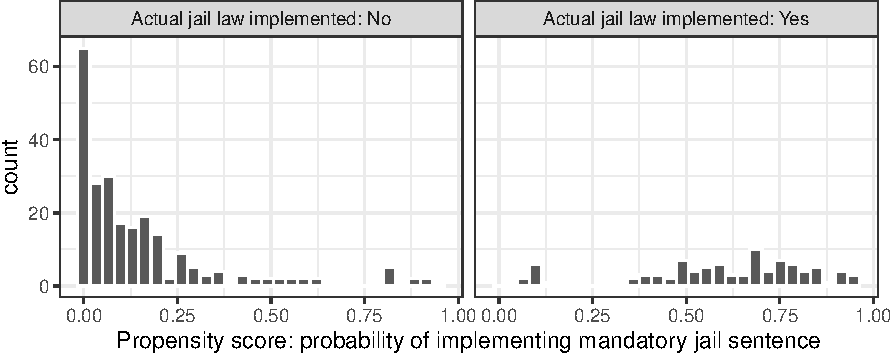
\includegraphics{team6_final_project_3_files/figure-latex/two-1} 

}

\caption{Propensity score distribution across two treatment groups before matching}\label{fig:two}
\end{figure}

\hypertarget{matching-1}{%
\subsubsection{Matching}\label{matching-1}}

Nearest neighbor matching algorithm resulted in a new dataset of 188 entires, with 94 original entries with mandatory jail sentence matched with their respective non-treated entry with the most similar propensity score. Figure \ref{fig:three} shows that after the matching procedure the propensity scores are more similarly distributed in the two treatment classes than the original dataset. Figure @ref(fig:cov\_bp) shows that distributions of the covariates are similar between treatments.

\begin{figure}

{\centering 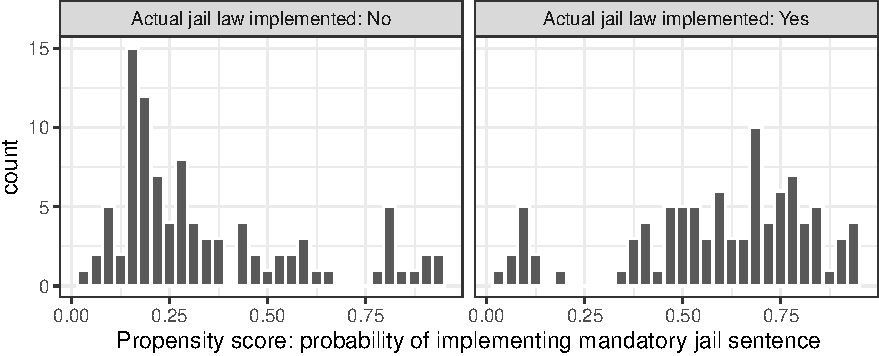
\includegraphics{team6_final_project_3_files/figure-latex/three-1} 

}

\caption{Propensity score distribution across two treatment groups after matching}\label{fig:three}
\end{figure}

\begin{figure}
\centering
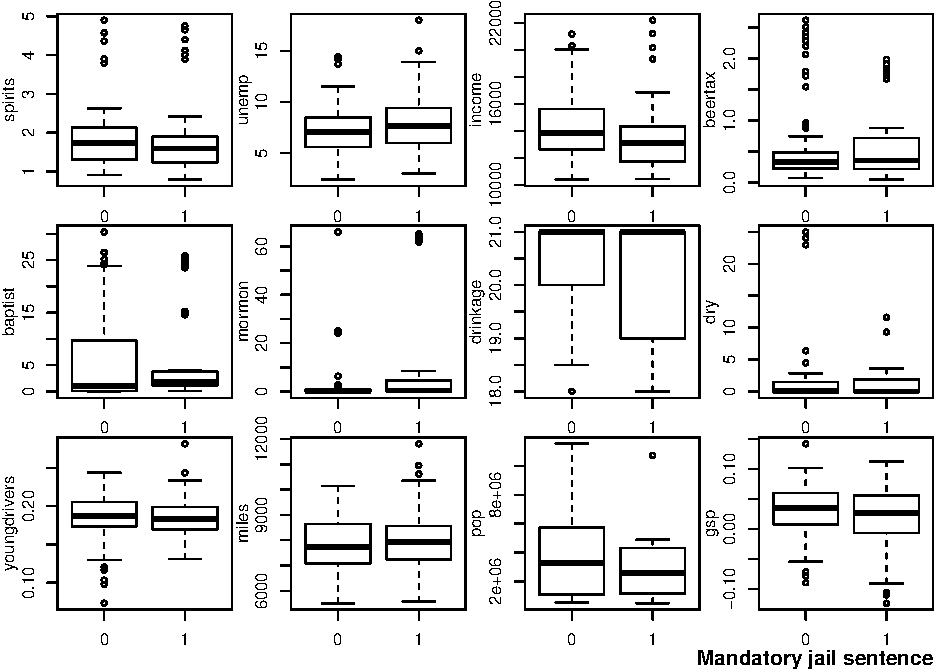
\includegraphics{team6_final_project_3_files/figure-latex/cov_bp-1.pdf}
\caption{(\#fig:cov\_bp)Distributions of the covariates after propensity score matching}
\end{figure}

\hypertarget{estimating-treatment-effect-1}{%
\subsection{Estimating Treatment Effect}\label{estimating-treatment-effect-1}}

\hypertarget{model-diagnostics-1}{%
\subsubsection{Model Diagnostics}\label{model-diagnostics-1}}

\hypertarget{fixed-effect-model}{%
\paragraph{Fixed Effect Model}\label{fixed-effect-model}}

The two crucial assumptions for a linear fixed effect model are the normal distribution and constant variance of the residuals across the fitted values. Influential observations will also be discussed.

\begin{figure}
\centering
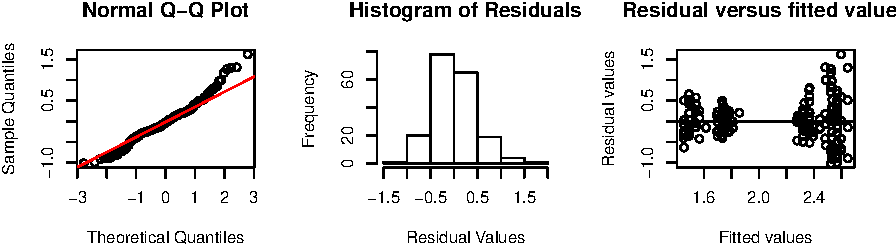
\includegraphics{team6_final_project_3_files/figure-latex/diag-1.pdf}
\caption{\label{fig:diag}Visual diagnostics of Fixed Effect model assumptions. (a). Normal Q-Q plot of residuals. (b) Histogram of model residuals. (c) Residuals-versus-fitted value scatter plot.}
\end{figure}

\hypertarget{normality-and-equal-variance}{%
\paragraph{Normality and Equal Variance}\label{normality-and-equal-variance}}

From the Q-Q plot of the residuals (Figure \ref{fig:diag} (a)), we can see that the probability mass on the left and right tails are higher than what is expected from a normal distribution. The distribution of the residuals seem to be heavy-tailed. Thus, the normality assumption is not satisfied from the Q-Q plot. A histogram is used to visualize the distribution of the residuals (Figure \ref{fig:diag} (b)). Figure \ref{fig:diag} A Shapiro-Wilk normality test yielded p = 0.002183, rejecting the null hypothesis that the residuals are normally distributed. (c) shows that the variance across residuals is not evenly distributed about mean zero.

\hypertarget{influential-observations}{%
\paragraph{Influential Observations:}\label{influential-observations}}

Since the Cook's distance for every observation is very small (the largest is less than 0.10), we conclude that there are no highly influential observations.

\hypertarget{response-variable-transformation}{%
\paragraph{Response Variable Transformation}\label{response-variable-transformation}}

In order to address the non-normally distributed residuals and non-constant residual variance, we performed box-cox transformation for the response variable with \(\lambda = 0\) (\(Y^{'} = logY\)).

\begin{figure}
\centering
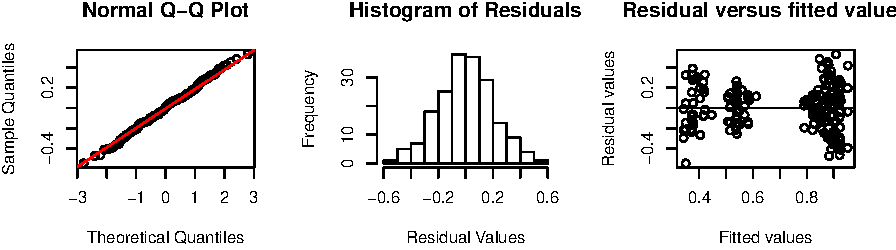
\includegraphics{team6_final_project_3_files/figure-latex/diag_log-1.pdf}
\caption{(\#fig:diag\_log)Visual diagnostics of Fixed Effect model assumptions with log transformed response variable. (a). Normal Q-Q plot of residuals. (b) Histogram of model residuals. (c) Residuals-versus-fitted value scatter plot.}
\end{figure}

\begin{verbatim}
## 
##  Shapiro-Wilk normality test
## 
## data:  residuals(fit4, type = "pearson")
## W = 0.99629, p-value = 0.9304
\end{verbatim}

The diagnostic diagrams of the fixed effect model with log-transformed fatality rate (Figure @ref(fig:diag\_log)) shows normally distributed residuals. A Shapiro-Wilk normality test yielded p = 0.9304, suggesting strong evidence for normally distributed residuals. The variance of the residuals is also much more constant than the original model.

\hypertarget{parameter-estimation}{%
\paragraph{Parameter estimation}\label{parameter-estimation}}

Table \ref{tab:fix} show the estimated values of the model parameters.

\begin{longtable}[]{@{}lllll@{}}
\caption{\label{tab:fix}Fixed effects of mandatory jail sentence}\tabularnewline
\toprule
Parameter & Estimate & Std. Error & t value & Pr(\textgreater{}\tabularnewline
\midrule
\endfirsthead
\toprule
Parameter & Estimate & Std. Error & t value & Pr(\textgreater{}\tabularnewline
\midrule
\endhead
Intercept & 0.56834 & 0.05508 & 10.319 & \textless{} 2 \(\times 10^{-16}\)\tabularnewline
jail & 0.04304 & 0.03268 & 1.317 & 0.189593\tabularnewline
\bottomrule
\end{longtable}

\begin{longtable}[]{@{}llllll@{}}
\caption{\label{tab:anova}Analysis of Variance Table}\tabularnewline
\toprule
Variance component & Df & Sum Sq & Mean Sq & F value & Pr(\textgreater{}F)\tabularnewline
\midrule
\endfirsthead
\toprule
Variance component & Df & Sum Sq & Mean Sq & F value & Pr(\textgreater{}F)\tabularnewline
\midrule
\endhead
jail & 1 & 0.0758 & 0.07579 & 1.7341 & 0.1896\tabularnewline
\bottomrule
\end{longtable}

To test whether mandatory jail sentence has significant effect on vehicle fatality rate, we fitted a reduced model with only fixed effects of region and time:

\[
Y_{ijl} = \mu + \alpha_i + \beta_j + \epsilon_{ijl}
\]

for \(i \in [Northeast, Midwest, South, West],\) \(j \in [1982, 1983, ..., 1988],\) \(k \in [0, 1],\) and \(l \in [1, ..., n_{ijk}]\).

Where\\
- \(Y_{ijl}\) represents the yearly traffic fatality rate of a given state in a given year.\\
- \(\mu\) represents the overall sample mean of fatality rates.\\
- \(\alpha_i\) represents the fixed effect of geographical region \(i\).\\
- \(\beta_j\) represents the fixed effect of year. Note that year is treated as a categorical variable, not a numerical variable.\\
- \(\epsilon_{ijl}\) is the error.

We used a Chi-squared test to test the following hypotheses:\\
\(H_0\): mandatory jail sentence has no significant effect on vehicle fatality rate (\(\gamma_0 = \gamma_1\) in full model);\\
\(H_1\): mandatory jail sentence has significant effect on vehicle fatality rate (\(\gamma_0 \neq \gamma_1\) in full model).

\begin{longtable}[]{@{}llllll@{}}
\caption{\label{tab:chisq}Chi-squared test of fixed effect}\tabularnewline
\toprule
Model & Residual Df & RSS & Df & Sum of Sq & Pr(\textgreater{}Chi)\tabularnewline
\midrule
\endfirsthead
\toprule
Model & Residual Df & RSS & Df & Sum of Sq & Pr(\textgreater{}Chi)\tabularnewline
\midrule
\endhead
Full & 177 & 7.7361 & & &\tabularnewline
Reduced & 178 & 7.8119 & -1 & -0.075792 & 0.1879\tabularnewline
\bottomrule
\end{longtable}

The p value suggests that we cannot reject null hypothesis that mandatory jail sentence does not have significant effect on vehicle fatality rate at \(\alpha = 0.05\).

\hypertarget{horvitz-thompson-inverse-probability-weighting-1}{%
\subsubsection{Horvitz-Thompson Inverse-Probability Weighting}\label{horvitz-thompson-inverse-probability-weighting-1}}

The Horvitz-Thompson inverse-probability weighting calculated ATE is \(\hat{\tau}^{ATE} = 0.096\). This number can be interpreted as the average effect of implementing mandatory jail sentence is increasing per 10K capita traffice fatality rate by 0.095.

\hypertarget{discussion}{%
\section{Discussion}\label{discussion}}

\hypertarget{propensity-score-matching}{%
\subsection{Propensity Score Matching}\label{propensity-score-matching}}

In this report, we highlight the usage of propensity score matching for isolating average treatment effect of implementing mandatory jail sentence. Rosenbaum and Rubin (1983) defined treatment assignment to be strongly ignorable if the following two conditions hold: (a) treatment assignment is independent of the potential outcomes conditional on the observed baseline covariates, and (b) every subject has a nonzero probability to receive either treatment. They demonstrated that if treatment assignment is strongly ignorable, conditioning on the propensity score allows one to obtain unbiased estimates of average treatment effects. We achieved these conditions through propensity score matching.

\hypertarget{horvitz-thompson-inverse-probability-weighting-2}{%
\subsection{Horvitz-Thompson Inverse-Probability Weighting}\label{horvitz-thompson-inverse-probability-weighting-2}}

The Horvitz-Thompson inverse-probability weighting method provides a direct estimate of average treatment effect of implementing mandatory jail sentence on traffic fatality rate. The result indicates that the mandatory jail sentence treatment has a very small (0.096 per 10,000 in population) effect in increasing traffic fatality rate, assuming the assumptions for causal inference hold true. Please see the following section for a comprehensive list of assumptions for causal inference.

\hypertarget{causal-inference}{%
\subsection{Causal Inference}\label{causal-inference}}

We cannot confidently draw causal conclusions using the result from this analysis. This is because of the violation of these assumptions necessary for causal inference:

\begin{enumerate}
\def\labelenumi{\arabic{enumi}.}
\item
  The stable unit treatment value assumption (SUTVA):\\
  SUTVA states that the treatment assignment of one experimental unit cannot interfere with the outcome of a separate experimental unit. This is violated in this dataset because temporal correlations across records taken from the same State, and spacial correlations among states that are geographically close to each other.
\item
  Exogeneity: The exogeneity assumption states that the independent variable (implementation of mandatory jail sentence) cannot be dependent on the dependent variable (vehicle fatality rate). This assumption is likely to be violated in this dataset because legislations can arise from existing conditions (Figure \ref{fig:dag} (a)).
\end{enumerate}

3.Observation of all Covariates: Although this expansive dataset captures many prominent variables that are associated with vehicle fatality rate, many more economic and social factors come into play in impacting the interactions between the implementation of mandatory jail sentence and vehicle fatality rate. We cannot confidently exclude the possiblity of the existence of many of such variables (Figure \ref{fig:dag} (b)).

\begin{figure}
\centering
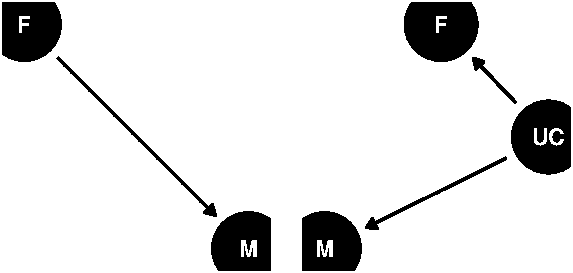
\includegraphics{team6_final_project_3_files/figure-latex/dag-1.pdf}
\caption{\label{fig:dag}Directed acyclic graphs of scenarios where direction of causal inference changes. a. Violation of exogeneity. b. Violation of ignorability of unobserved confounding variables. M: mandatory jail sentence; F: vehicle fatality rate; UC: unobserved confounding variable}
\end{figure}

Ultimately, our analysis makes very improbable assumptions in order to analyze this observational data. Due to this lack of strong assumptions around SUTVA and observation of all covariates, we fail to make any strong causal conclusions regarding the effect of mandatory jail sentences on State fatality rates.\\
Due to this lack of clear causality, we propose State legislators focus their energy and capital on measures directly correlated with the probability of entering a fatal collision. Better seatbelt enforcement, speeding enforcement, and drunk driver intervention have all demonstrated their effectiveness at better-protecting citizens and reducing the risk of a fatal accident (Morley, 2016). Legislators should focus on active measures to combat fatal automobile collisions instead of hoping to find a strong causal effect in passive measures like mandatory jail sentencing.

\hypertarget{references}{%
\section{References}\label{references}}

Austin P. C. (2011). An Introduction to Propensity Score Methods for Reducing the Effects of Confounding in Observational Studies. Multivariate behavioral research, 46(3), 399--424. \url{doi:10.1080/00273171.2011.568786}

Brookhart M.A., Schneeweiss S., Rothman K.J., Glynn R.J., Avorn J., Stürmer T. (2006). Variable selection for propensity score models. American Journal of Epidemiology. 163, 1149--1156.\\
Rosenbaum P.R., Rubin D.B. (1983). The central role of the propensity score in observational studies for causal effects. Biometrika. 70:41--55.

Durbin, D. R., Elliott, M. R., \& Winston, F. K. (2009). A propensity score approach to estimating child restraint effectiveness in preventing mortality. Statistics and Its Interface, 2(4), 437--447. doi: 10.4310/sii.2009.v2.n4.a5

Horvitz, D. G., \& Thompson, D. J. (1952). A generalization of sampling without replacement from a finite universe. Journal of the American statistical Association, 47(260), 663-685.

Morley, A., Morris, A., Abi Semaan, M., \& Hancox, G. (2016). A Guide for Policy Makers: On Reducing Road Fatalities. Retrieved from \url{https://www.pwc.com/m1/en/publications/guide-on-reducing-road-fatalities.html}

Rodriguez, D., Rejesus, R., \& Aragon, C. (2007). Impacts of an Agricultural Development Program for Poor Coconut Producers in the Philippines: An Approach Using Panel Data and Propensity Score Matching Techniques. Journal of Agricultural and Resource Economics, 32(3), 534-557. Retrieved February 14, 2020, from www.jstor.org/stable/40982695

Rosenbaum, P., \& Rubin, D. (1983). The Central Role of the Propensity Score in Observational Studies for Causal Effects. Biometrika, 70(1), 41-55. \url{doi:10.2307/2335942}

Sasidharan, L., \& Donnell, E. T. (2013). Application of propensity scores and potential outcomes to estimate effectiveness of traffic safety countermeasures: Exploratory analysis using intersection lighting data. Accident Analysis \& Prevention, 50, 539--553. doi: 10.1016/j.aap.2012.05.036

Smith, H. L. (1997). 6. Matching with Multiple Controls to Estimate Treatment Effects in Observational Studies. Sociological methodology, 27(1), 325-353.

\end{document}
